%%!TEX root = ./UserManual.tex
\chapter{Visualiser}
\label{chap:visualiser}


%%%%%%%%%%%%%%%%%%%%%%%%%%%%%%%%%%%%%%%%%%%%%%%%%%%%%%%%%%%%%%%%
% Overview
%%%%%%%%%%%%%%%%%%%%%%%%%%%%%%%%%%%%%%%%%%%%%%%%%%%%%%%%%%%%%%%%
\section{Overview}
\label{section:overview}

\paragraph{} The Stride software includes a visualisation tool with which the disease spreading can be shown on a geographical map. When the visualiser is opened, the user is presented with a geographical map, a sidebar to the left and a toolbar on top. An overview can be seen in figure \ref{fig:screenshot_overview}

The toolbar contains various controls:
\begin{itemize}
\item Open file: Opens a open file dialog.
\item Save file: Opens a save to image file dialog.
\item Select Radius: Opens the radius selection dialog.
\item Select Rectangle: Opens the rectangle selection dialog.
\item Play-button: Enables/disables the automatic playback of the simulation results.
\item Timestep-slider: Allows the user to select a certain timestep of the simulation.
\item Health status dropdown: Allows the user to select a health status that is to be displayed.
\end{itemize}

%%%% IMAGE: overview

\begin{figure}[H]
\centering
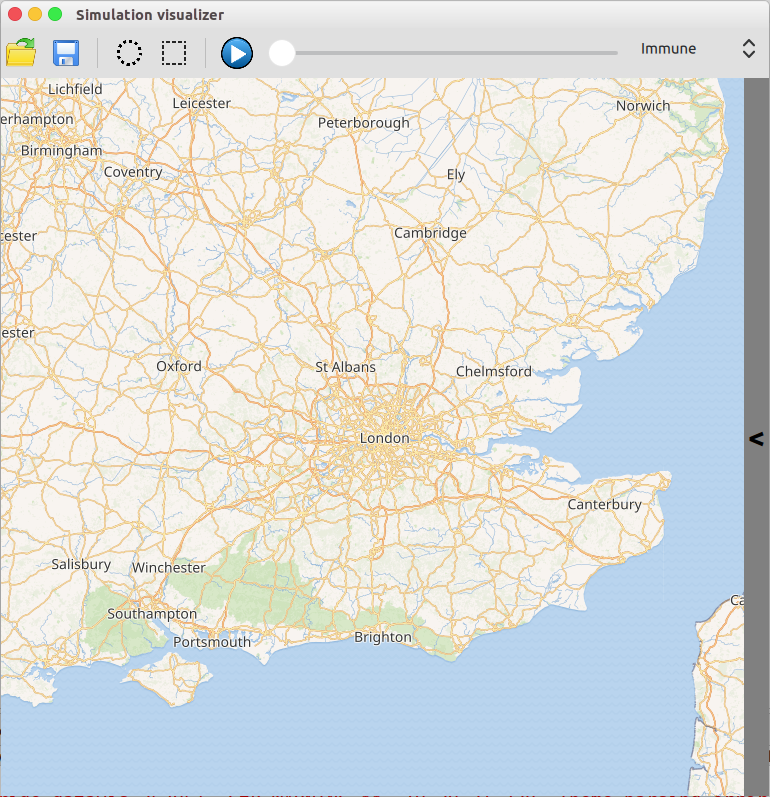
\includegraphics[width=0.7\textwidth,keepaspectratio]{images/overview.png}
\label{fig:screenshot_overview}
\caption{Overview of the visualisation tool}
\end{figure}

%%%%%%%%%%%%%%%%%%%%%%%%%%%%%%%%%%%%%%%%%%%%%%%%%%%%%%%%%%%%%%%%
% Viewing simulations
%%%%%%%%%%%%%%%%%%%%%%%%%%%%%%%%%%%%%%%%%%%%%%%%%%%%%%%%%%%%%%%
\section{Viewing simulations}
\label{section:viewing}

%%% IMAGE: open file
\begin{figure}[H]
\centering
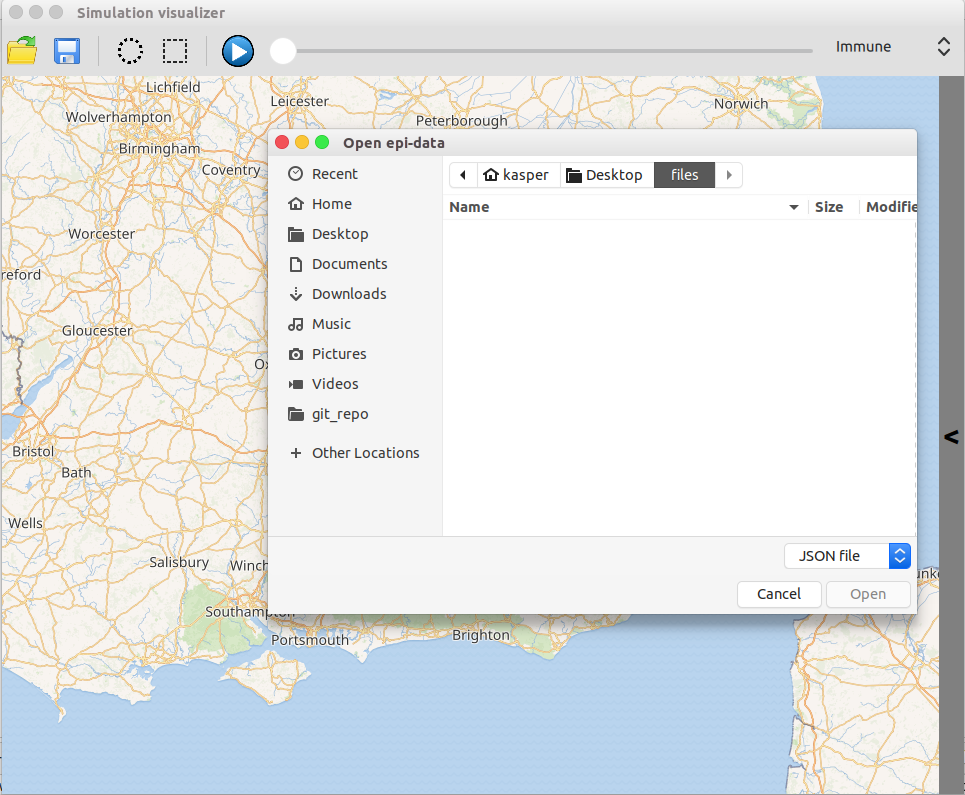
\includegraphics[width=0.7\textwidth,keepaspectratio]{images/open_file.png}
\label{fig:screenshot_openFile}
\caption{The open file dialog}
\end{figure}

%%% IMAGE: view simulation
\begin{figure}[H]
\centering
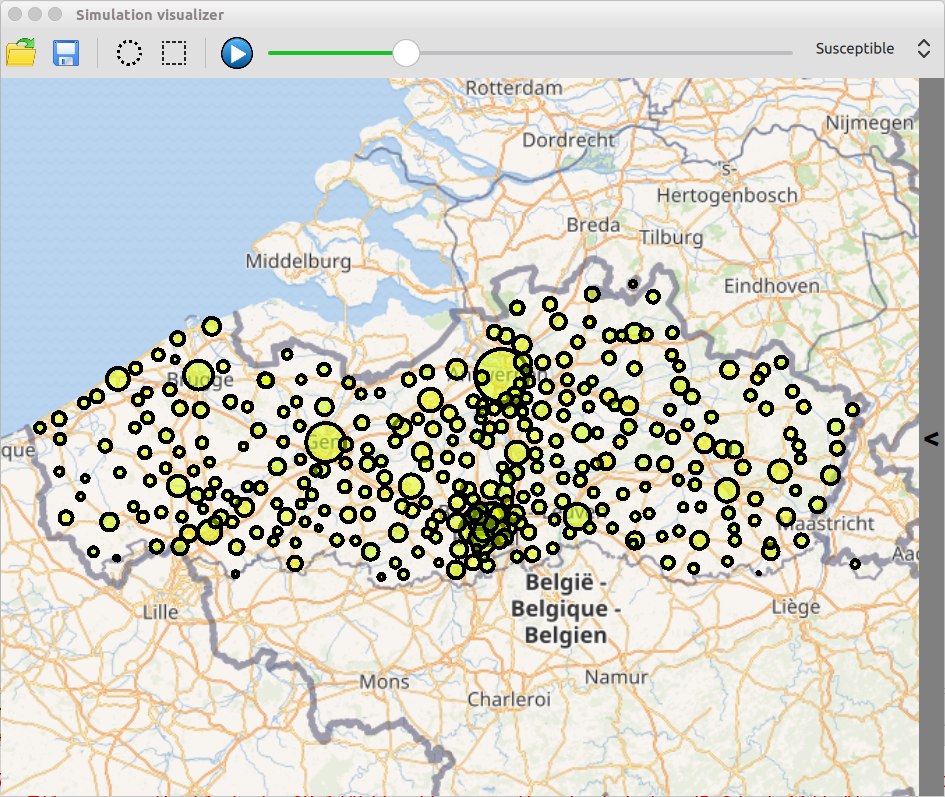
\includegraphics[width=0.7\textwidth,keepaspectratio]{images/view_simul.png}
\label{fig:screenshot_viewSimul}
\caption{The visualiser after a simulation has been opened}
\end{figure}



%%%%%%%%%%%%%%%%%%%%%%%%%%%%%%%%%%%%%%%%%%%%%%%%%%%%%%%%%%%%%%%%
% Selecting and viewing statistics
%%%%%%%%%%%%%%%%%%%%%%%%%%%%%%%%%%%%%%%%%%%%%%%%%%%%%%%%%%%%%%%
\section{Selecting and viewing statistics}
\label{section:stats_selection}

%%% IMAGE: view location stats
\begin{figure}[H]
\centering
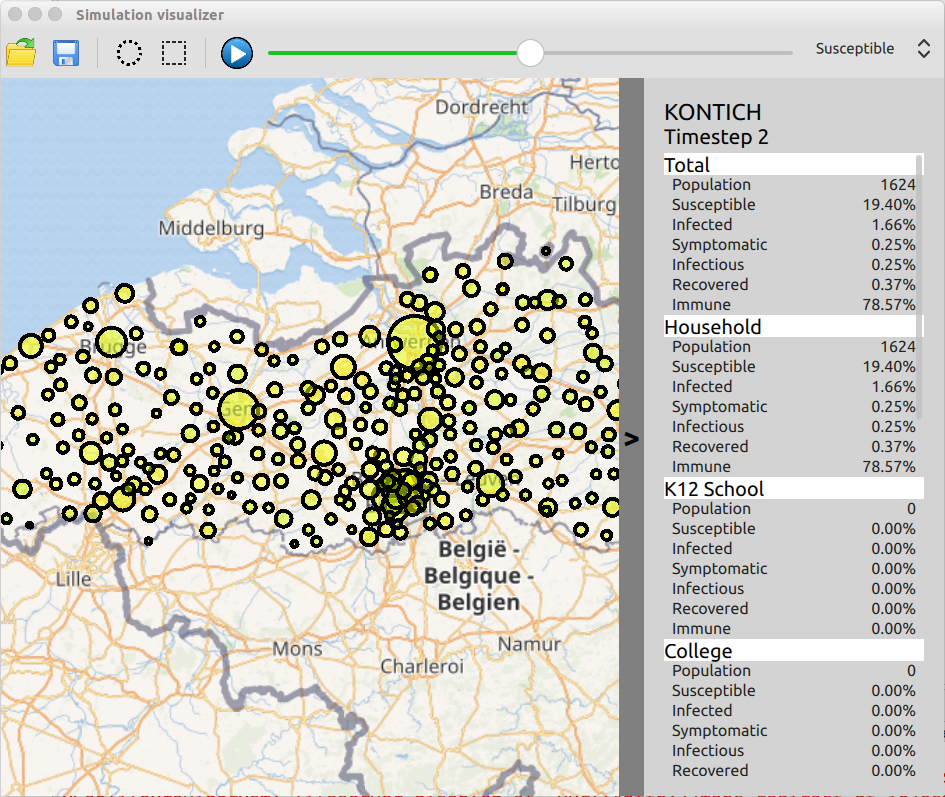
\includegraphics[width=0.7\textwidth,keepaspectratio]{images/stats_loc.png}
\label{fig:sceenshot_statsLoc}
\caption{The sidebar displaying statistics for the clicked location}
\end{figure}

%%% IMAGE rad selection
\begin{figure}[H]
\centering
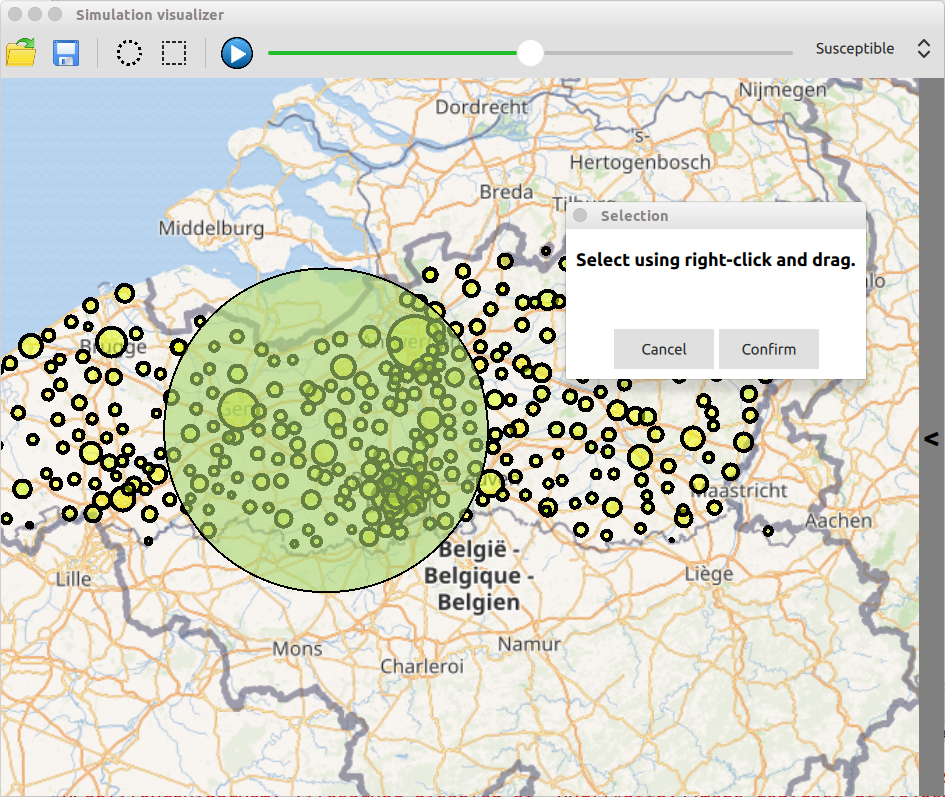
\includegraphics[width=0.7\textwidth,keepaspectratio]{images/select_rad.png}
\label{fig:screenshot_selectRad}
\caption{Radius selection}
\end{figure}

%%% IMAGE rect selection
\begin{figure}[H]
\centering
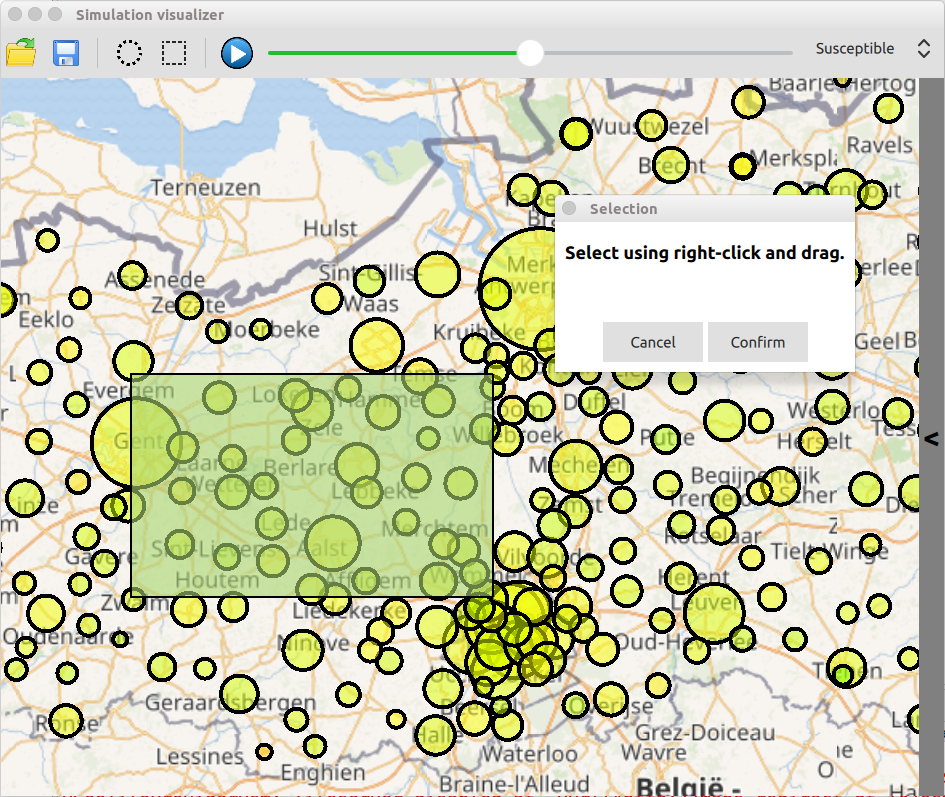
\includegraphics[width=0.7\textwidth,keepaspectratio]{images/select_rect.png}
\label{fig:screenshot_selectRect}
\caption{Rectangular selection}
\end{figure}


%%%%%%%%%%%%%%%%%%%%%%%%%%%%%%%%%%%%%%%%%%%%%%%%%%%%%%%%%%%%%%%%
% Exporting to image
%%%%%%%%%%%%%%%%%%%%%%%%%%%%%%%%%%%%%%%%%%%%%%%%%%%%%%%%%%%%%%%%

%%% IMAGE save to selection

\section{Exporting to image}
\label{section:export_image}


